\section{An Example of Proof Refactoring}
\label{sec:overview}

\begin{figure}
\begin{minipage}{0.46\textwidth}
   \lstinputlisting[firstline=1, lastline=3]{listswap.tex}
\end{minipage}
\hfill
\begin{minipage}{0.46\textwidth}
   \lstinputlisting[firstline=5, lastline=7]{listswap.tex}
\end{minipage}
\caption{The updated \lstinline{list} (right) is the old \lstinline{list} (left) with its two constructors swapped (\codediff{orange}).}
\label{fig:listswap}
\end{figure}

\toolname is a tool for proof refactoring and repair that is available on Github.\footnote{Link withheld for double-blind review.}
Consider a simple example of using \toolname: refactoring list proofs after swapping the two constructors of a list (Figure~\ref{fig:listswap}).
Even such a simple change can quickly cause trouble in existing proofs, like this proof from the Coq standard library:\footnote{Here and throughout, we use induction instead of pattern matching.}

\begin{lstlisting}
Lemma rev_app_distr {A : Type} :
  $\forall$ (x y : list A), rev (x ++ y) = rev y ++ rev x.
Proof.
  induction x as [| a l IHl].
  induction y as [| a l IHl].
  simpl. auto.
  simpl. rewrite app_nil_r; auto.
  intro y. simpl.
  rewrite (IHl y). rewrite app_assoc; trivial.
Qed.
\end{lstlisting}
This theorem says that appending two lists and reversing the result behaves the same way as appending
the reverse of the second list onto the reverse of the first list.
This theorem statement \lstinline{rev_app_distr} defined over the old version of \lstinline{list} is our \textit{old specification}.
When we change the \lstinline{list} type, we get the \textit{new specification}.
But the \textit{old proof} or tactic script no longer works with this new specification.

To update the proof script with \toolname, all we need to do is run this command (here and throughout, we use $\codeauto{light blue}$ to denote
functions and proofs that \toolname produces automatically):

\begin{lstlisting}
Repair Old.list New.list in rev_app_distr.
\end{lstlisting}
assuming our old and new list types are in separate modules called \lstinline{Old} and \lstinline{New}.
This produces a refactored proof script:

\begin{lstlisting}
Lemma (@\codeauto{rev_app_distr}@) {A : Type} :
  forall (x y : list A), rev (x ++ y) = rev y ++ rev x.
Proof.
  intros x y. revert y. induction x as [a l IHl|].
  - intro y0. simpl.
    rewrite (IHl y0). simpl. rewrite (app_assoc (rev y0) (rev l) (a::[])). reflexivity.
  - intro y0. induction y0 as [a l IHl|].
    + simpl. rewrite (app_nil_r (rev l) (a::[])). reflexivity.
    + reflexivity.
Qed.
\end{lstlisting}
where all of the dependencies---\lstinline{rev}, \lstinline{++}, \lstinline{app_assoc}, and \lstinline{app_nil_r}---have
also been refactored automatically.
If we'd like, we can manually tweak this to something that more closely matches the original:

\begin{lstlisting}
Proof.
  induction x as [a l IHl|].
  intro y. simpl.
  rewrite (IHl y). rewrite (@\codeauto{app_assoc}@); trivial.
  induction y as [a l IHl|].
  simpl. rewrite (@\codeauto{app_nil_r}@); auto.
  simpl. auto.
Qed.
\end{lstlisting}
We can even refactor the entire list module all at once by running the \lstinline{Repair module}
command; the results of this are in \lstinline{Swap.v}.\footnote{Link withheld for double-blind review.} % TODO

\paragraph{Configure, Transform, Decompile}
The key to success here is that \toolname does not even attempt to refactor the poorly structured proof script directly.
Even for the simple proof script above, this would not be straightforward: Grouping tactics by line, there are $6! = 620$
permutations of this proof script.
It is not clear which lines to swap since these tactics do not have a semantics beyond the meaning imposed by evaluating them.
Furthermore, just swapping lines is not enough: even for a simple refactoring, we must also swap
arguments, so that \lstinline{induction x as [| a l IHl]} becomes \lstinline{induction x as [a l IHl|]}.
Handling even swapping constructors this way would require a specific search procedure that would not generalize to other changes.
\citep{robert2018} describes the challenges of refactoring tactics directly in detail.

Instead, \toolname takes advantage of the fact that Coq's \textit{proof term} language Gallina is well structured.
Coq compiles each proof script to a proof term---\toolname repairs that term.
\toolname then decompiles the repaired proof term back to a proof script that the user can maintain.

\begin{figure}
\begin{minipage}{0.49\textwidth}
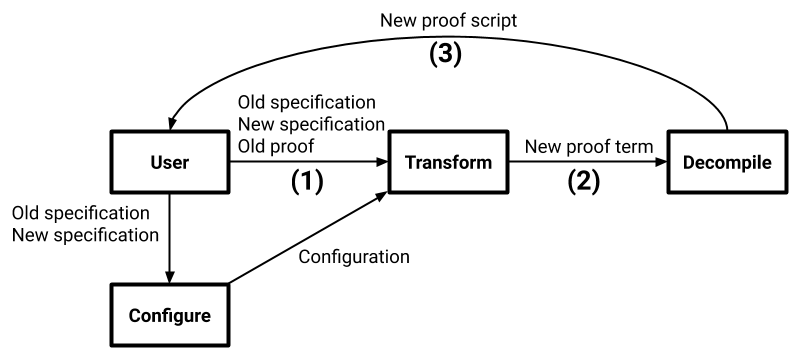
\includegraphics[width=\linewidth]{workflowa.png}
\end{minipage}
\hfill
\begin{minipage}{0.49\textwidth}
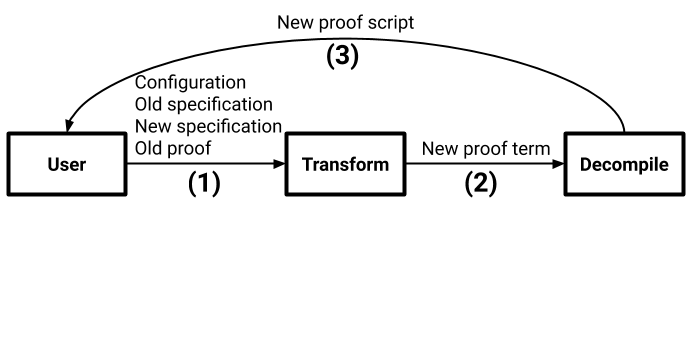
\includegraphics[width=\linewidth]{workflowb.png}
\end{minipage}
\caption{The two possible workflows for \toolname, using either automatic (left) or manual (right) configuration.}
\label{fig:system}
\end{figure}

The repair step works using a configurable program transformation.
This program transformation transforms the old proof term into a new proof term that refers to the new specification
(here, the theorem that refers to \lstinline{New.list})
in place of the old specification (here, the theorem that refers to \lstinline{Old.list}),
and otherwise preserves the behavior of the old proof term.
The configuration instantiates the program transformation to the old and new specifications (here, \lstinline{Old.list} and \lstinline{New.list})
so that it knows how to preserve behavior modulo that change.
Figure~\ref{fig:system} shows how this comes together when the user invokes \toolname:

\begin{enumerate}
\item \toolname configures itself, either:
\begin{enumerate}
\item automatically (left), using \textbf{Configure} to discover the configuration, or
\item manually (right), by taking the configuration as an argument.
\end{enumerate}
\item The configured \textbf{Transform} transforms the old proof term into the new proof term.
\item \textbf{Decompile} produces a new proof script from the new proof term.
\end{enumerate}

Our example uses automatic configuration. When we run the \lstinline{Repair} command:

\begin{lstlisting}
Repair Old.list New.list in rev_app_distr.
\end{lstlisting}
\textbf{Configure} invokes a special search procedure that automatically discovers that \lstinline{New.list}
is just \lstinline{Old.list} with a single moved constructor.
The search procedure proves an equivalence between \lstinline{Old.list} and \lstinline{New.list},
then configures \textbf{Transform} using that equivalence.
\textbf{Transform} then ports the proof term that inducted over \lstinline{Old.list}
to instead induct over \lstinline{New.list}, and finally
\textbf{Decompile} produces the tactic script that we see.

While this is a simple refactoring, this same workflow can get us much more.
Section~\ref{sec:search} shows how we have used \toolname to support industrial integration with Coq,
write dependently-typed functions and proofs with little user effort,
support examples from a benchmark from Coq proof engineers,
and port proofs between unary and binary natural numbers.

